\section{Desarrollo tecnológico y estado del prototipo}

\subsection{Arquitectura implementada}

Pulso se organizó en tres partes: las pantallas, el servidor que procesa las
acciones y la base de datos. Las pantallas utilizan React y
TypeScript; React facilita organizar las pantallas mediante componentes
reutilizables \parencite{react2026}. El backend emplea Django 5.1 y Django REST
Framework para los modelos, la autenticación, la validación y la API
\parencite{django51,drf315}. PostgreSQL almacena los datos en Supabase.

Para tareas en segundo plano se prepararon Celery y Redis. Estas herramientas
permiten enviar un trabajo a una cola y ejecutarlo por separado
\parencite{celery2026}. En el equipo de desarrollo se ejecutan con Docker
Compose. Su funcionamiento continuo está pendiente en la demostración de Vercel.

\begin{table}[htbp]
\caption{Tecnologías utilizadas en Pulso}
\begin{tabularx}{\textwidth}{>{\bfseries}p{3cm}p{4cm}X}
\toprule
Capa & Tecnología & Uso en Pulso \\
\midrule
Frontend & React 18, TypeScript, Vite 5 & SPA responsive, rutas, formularios y vistas por rol. \\
Interfaz & Tailwind CSS, Recharts, Lucide & Estilos, gráficos e iconografía. \\
Estado y datos & TanStack Query, Zustand, Axios & Caché de servidor, sesión y comunicación HTTP. \\
Backend & Django 5.1, DRF 3.15 & Reglas de negocio, permisos y API REST. \\
Autenticación & JWT y cookies HTTP-only & Inicio, renovación y cierre de sesión por rol. \\
Datos & PostgreSQL en Supabase & Persistencia relacional y migraciones. \\
Procesos & Celery, Celery Beat y Redis & Base técnica local para tareas asíncronas futuras. \\
Despliegue & Vercel y Docker & Demo pública y entornos reproducibles. \\
Pruebas & Pytest, Vitest y Playwright & Reglas backend, componentes y flujos de navegador. \\
\bottomrule
\end{tabularx}
\caption*{\textit{Nota}. Elaboración propia a partir del desarrollo de Pulso \parencite{gymhub_repo}.}
\end{table}

\subsection{Módulos funcionales}

La versión preparada para la etapa regional distingue tres contextos de acceso:
administrador, instructor y cliente. El administrador controla clientes, pagos y
asistencia; el instructor trabaja con los clientes asignados y sus planes de
entrenamiento; y el cliente consulta su membresía y sigue el programa asignado.
Una misma cuenta de demostración puede cambiar de contexto cuando tiene los
perfiles autorizados, sin que esto modifique los permisos de cada función.

Los planes de entrenamiento y la facturación se mantienen como procesos
separados. En la pestaña Planes, el entrenador crea la rutina, selecciona al
miembro, configura días y ejercicios, resuelve conflictos con un plan activo y
publica el programa. En Facturación se crea o renueva la membresía comercial, se
define precio y recurrencia, se registra el pago y se controla la vigencia o la
mora. La membresía define la vigencia del servicio del gimnasio; la rutina
indica qué ejercicios debe realizar el miembro.

\begin{longtable}{>{\bfseries}p{3.1cm}p{7.3cm}p{3.8cm}}
\caption{Estado de los módulos del MVP}\label{tab:modulos}\\
\toprule
Módulo & Capacidad observable & Estado y límite \\
\midrule
\endfirsthead
\toprule
Módulo & Capacidad observable & Estado y límite \\
\midrule
\endhead
Autenticación y contextos & Inicio, cierre, renovación y acceso de administrador, instructor o cliente. & Funcional; requiere operación segura de secretos y cookies. \\
Clientes & Registro, consulta, activación y relación con un instructor. & Administrador e instructor autorizado; los datos pertenecen a cuentas individuales. \\
Planes de entrenamiento & Creación y asignación desde Planes; días, ejercicios, estados y entrenamiento del día. & Instructor autorizado; separado de la membresía comercial. \\
Asistencia & Check-in e historial condicionado por el estado de la membresía. & Administrador y cliente según la tarea; el ingreso físico automatizado es futuro. \\
Progreso & Sesiones, registros de ejercicios y métricas básicas. & Funcional en el nivel del MVP. \\
Facturación & Catálogo de membresías, altas, renovaciones, pagos, vencimientos y mora. & Administrador controla la operación; el cliente consulta su membresía. No es contabilidad ni pasarela bancaria. \\
Perfil & Consulta y actualización de los datos permitidos de la cuenta. & Funcional según el rol autenticado. \\
\bottomrule
\caption*{\textit{Nota}. Estado funcional comprobado por el equipo en la versión local de demostración, 23 de septiembre de 2026.}
\end{longtable}

\subsection{Evidencia de funcionamiento}

Las pruebas revisaron el servidor, las pantallas y tareas completas desde el
navegador. Se comprobaron el inicio de sesión, el registro de miembros, la
activación de membresías, los pagos, la asistencia, las rutinas y el progreso.
Estas revisiones ayudan a encontrar errores antes de una demostración. Los
conteos y la fecha de las pruebas se presentan en los apéndices.

La interfaz, la API y su documentación cuentan con despliegues de demostración.
Durante la exposición se mostrará al jurado, con datos ficticios, el recorrido
del administrador para pagos y asistencia, el del instructor para configurar un
plan y el del cliente para seguir la rutina. La evidencia visual incluida se
limita a pantallas que coinciden con el alcance vigente.

\begin{figure}[htbp]
\centering
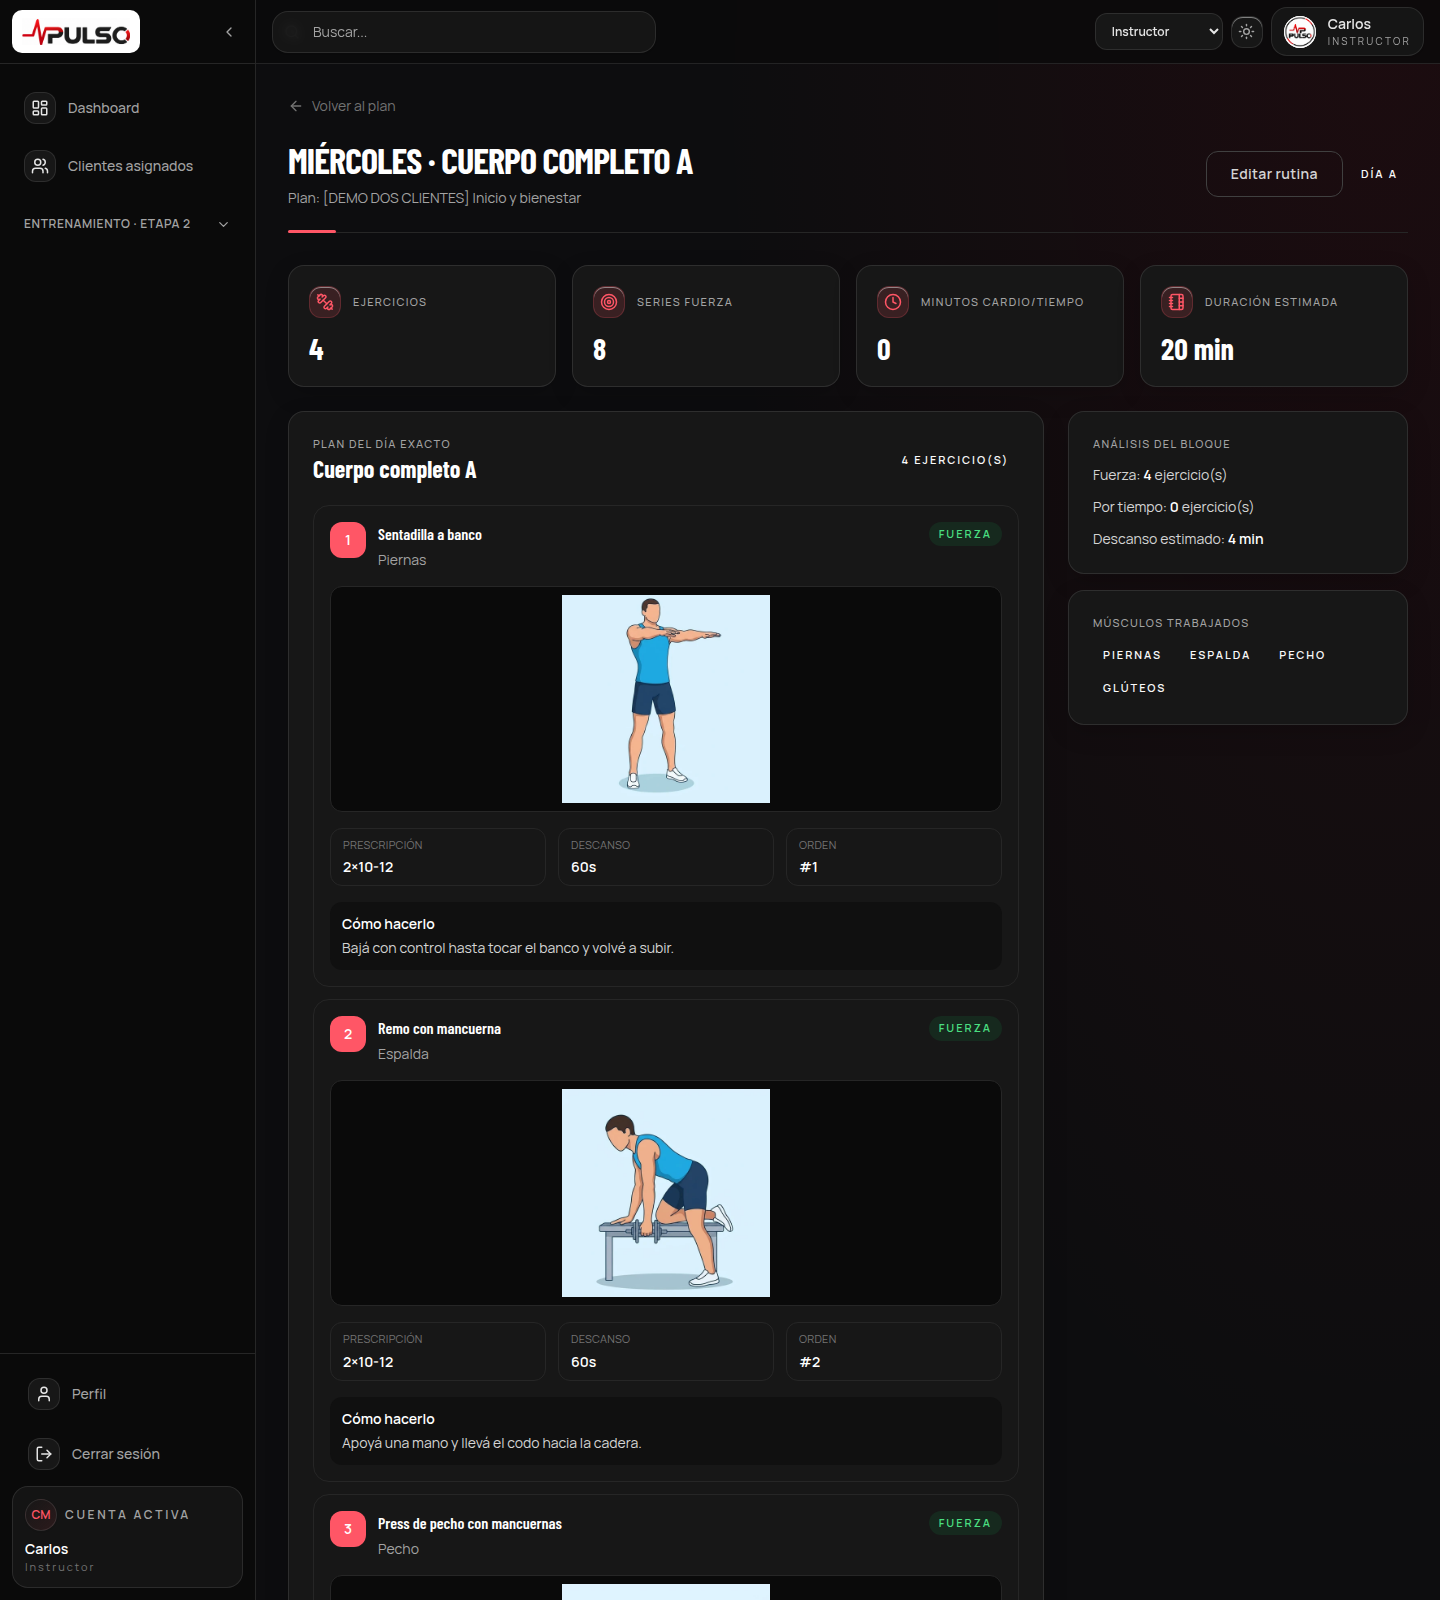
\includegraphics[width=0.92\textwidth]{imagenes/captura_actual_planes_instructor.png}
\caption{Configuración de un plan de entrenamiento por el instructor}
\label{fig:planes-instructor}
\caption*{\textit{Nota}. Captura propia de la versión local de demostración con datos ficticios, 23 de septiembre de 2026.}
\end{figure}

La Figura~\ref{fig:planes-instructor} muestra cómo la rutina se crea, asigna,
configura, finaliza o archiva desde Planes. La existencia de un plan deportivo
no implica que el miembro tenga una membresía comercial vigente.

\begin{figure}[htbp]
\centering
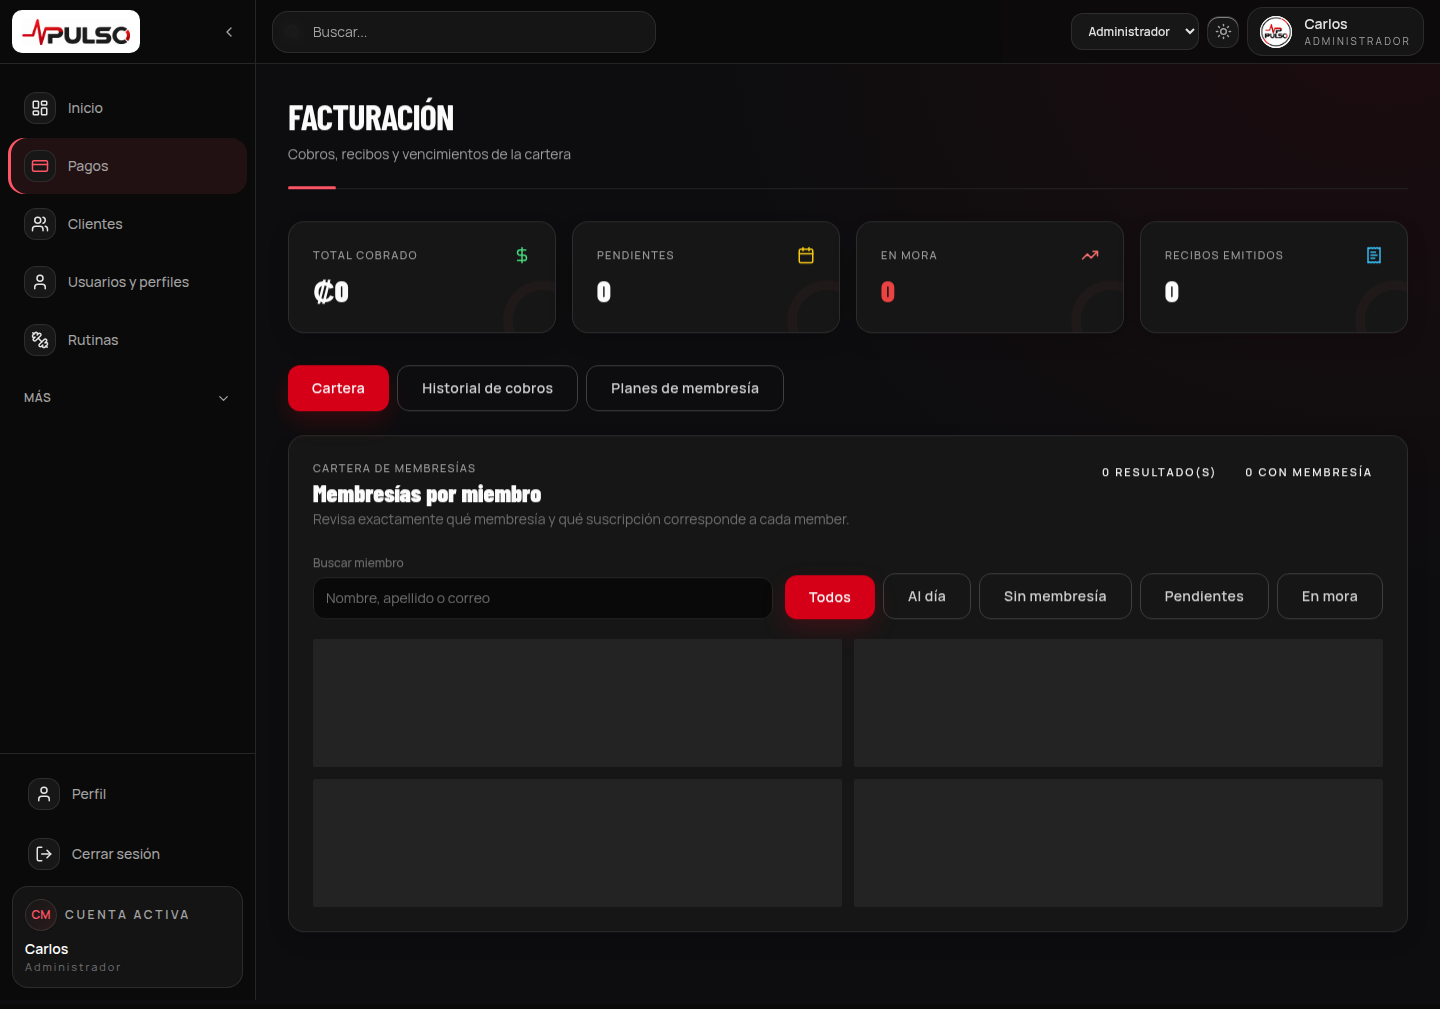
\includegraphics[width=0.92\textwidth]{imagenes/captura_actual_facturacion_administrador.png}
\caption{Cartera de membresías y pagos en Facturación}
\label{fig:facturacion-administrador}
\caption*{\textit{Nota}. Captura propia de la versión local de demostración con datos ficticios, 23 de septiembre de 2026.}
\end{figure}

La Figura~\ref{fig:facturacion-administrador} muestra la membresía de cada miembro,
su precio, vencimiento y pagos registrados. Los cobros se anotan en el sistema;
el procesamiento bancario y la contabilidad quedan fuera de esta función.

\begin{figure}[htbp]
\centering
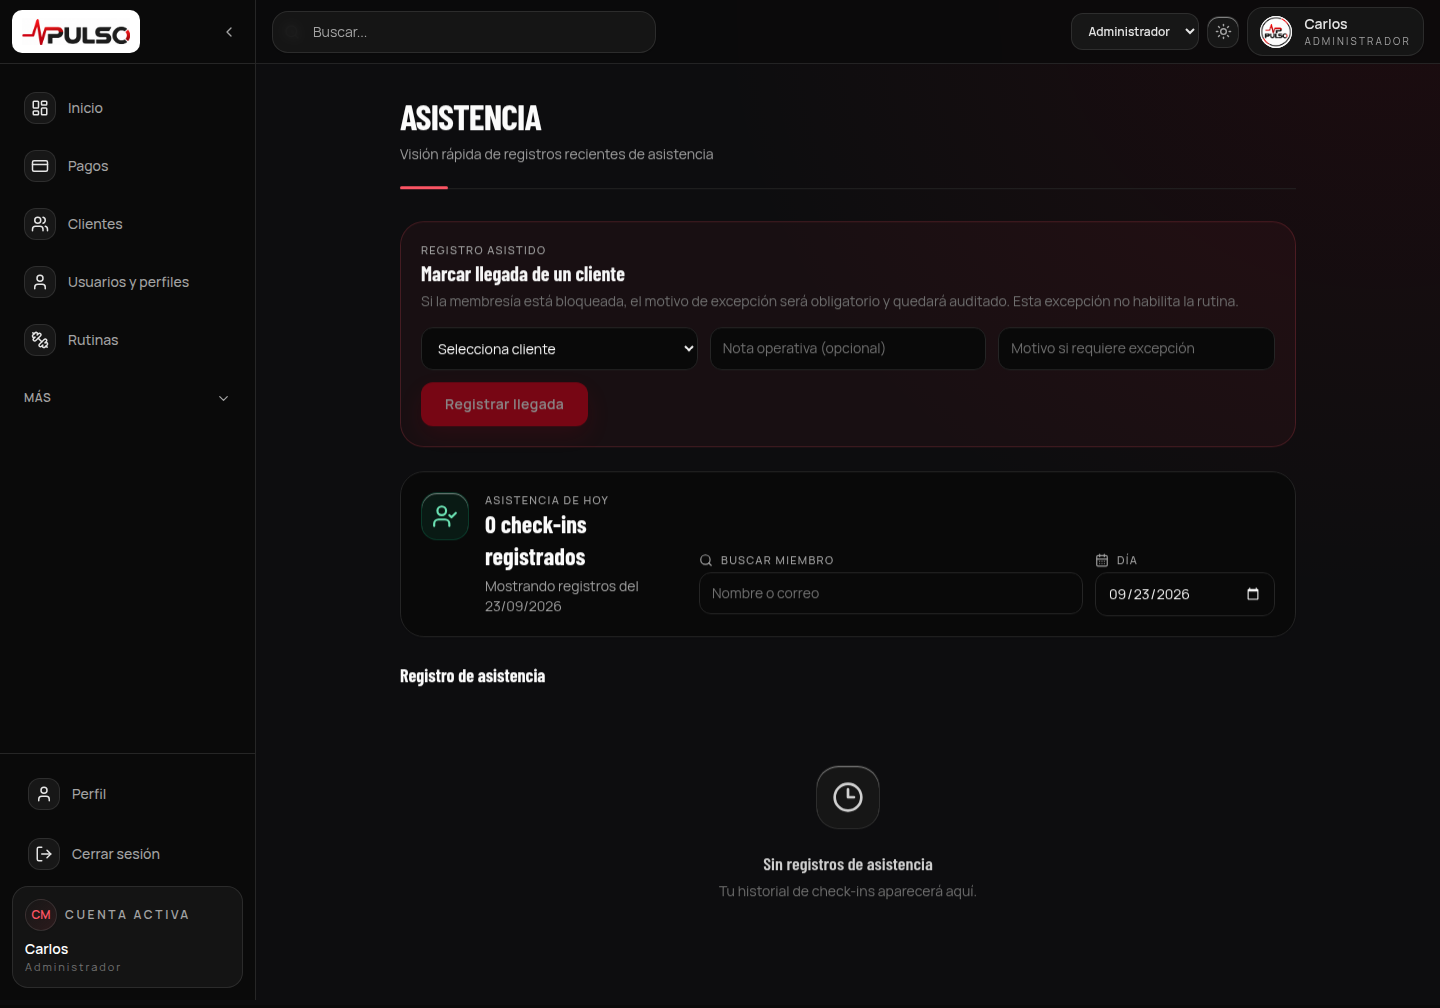
\includegraphics[width=0.92\textwidth]{imagenes/captura_actual_asistencia_administrador.png}
\caption{Consulta de asistencia desde el rol administrador}
\label{fig:asistencia-administrador}
\caption*{\textit{Nota}. Captura propia de la versión local de demostración con datos ficticios, 23 de septiembre de 2026.}
\end{figure}

La Figura~\ref{fig:asistencia-administrador} muestra la consulta por fecha y miembro.
El MVP registra check-in e historial; no controla por sí solo una puerta o torno
físico.

\begin{figure}[htbp]
\centering
\includegraphics[width=0.92\textwidth]{imagenes/captura_actual_rutina_miembro.png}
\caption{Rutina guiada para cliente}
\label{fig:rutina-miembro}
\caption*{\textit{Nota}. Captura propia de la versión local de demostración con datos ficticios, 23 de septiembre de 2026.}
\end{figure}

La Figura~\ref{fig:rutina-miembro} muestra el entrenamiento del día y las
decisiones guiadas disponibles para el cliente. La membresía, las indicaciones
del instructor y el progreso se consultan desde sus apartados correspondientes.

\subsection{Seguridad y privacidad}

El prototipo usa permisos por rol, cookies HTTP-only para JWT, controles CORS y
CSRF, y configuración separada por ambiente. Django incluye mecanismos para
autenticación, autorización y seguridad web \parencite{django51}. La existencia
de estos mecanismos se complementa con revisiones, actualizaciones, cambios de
claves y copias de seguridad.

El tratamiento de los datos de identidad, pagos, asistencia y progreso se regirá
por su finalidad, el consentimiento y el acceso autorizado. La Ley n.º 8968
aplica a bases de datos privadas y protege el control de las personas sobre su
información \parencite{ley8968}. Toda demostración utilizará datos ficticios o
anonimizados.

\subsection{Preparación para el piloto comercial}

La siguiente etapa técnica consiste en preparar una cuenta independiente para el
gimnasio piloto, configurar respaldos y
definir el procedimiento de soporte. También se implementará almacenamiento
persistente para archivos y una revisión completa de permisos antes de incorporar
datos reales.

Para crecer a varios clientes, cada gimnasio tendrá una entidad propia asociada
con sus miembros, entrenadores y registros. Las consultas y
permisos se limitarán al gimnasio autenticado. Esta separación también permitirá
configurar nombre, logo y colores, y obtener el conteo de membresías activas que
determina el plan comercial. Estas mejoras deben completarse antes de atender
varios gimnasios con datos reales en un mismo servicio.
